\documentclass[tikz,border=6pt]{standalone}
\usetikzlibrary{calc}
\begin{document}
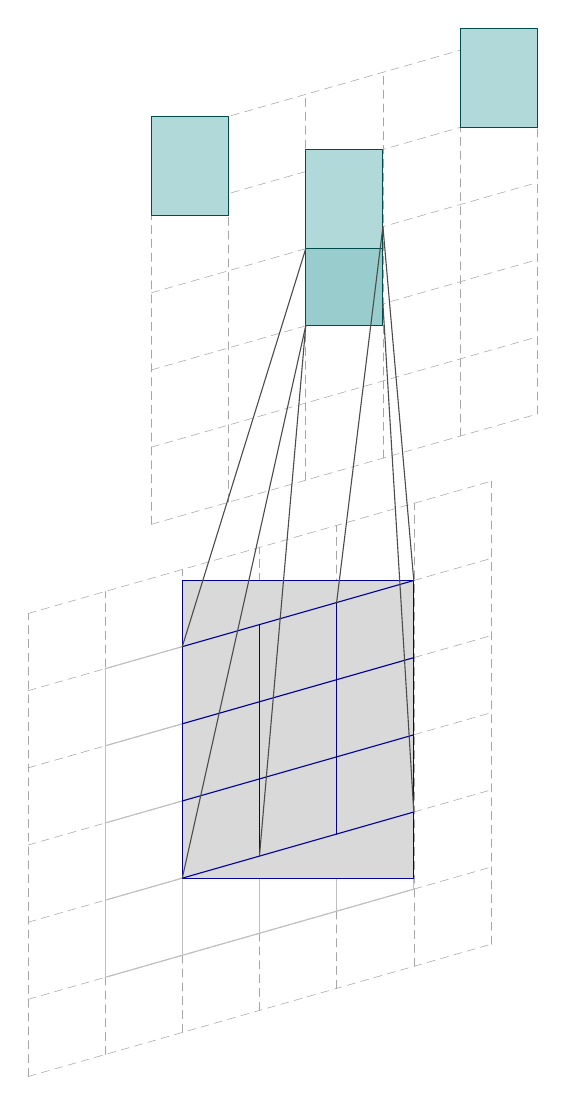
\begin{tikzpicture}[
  x={(0.98cm,0.28cm)}, y={(0cm,0.98cm)},
  every path/.style={line cap=round, line join=round}
]

% ---------------- Bottom feature map ----------------
\foreach \i in {-1,...,5} {
  \draw[densely dashed, gray!70, very thin] (-1,\i) -- (5,\i);
  \draw[densely dashed, gray!70, very thin] (\i,-1) -- (\i,5);
}
\foreach \i in {0,...,4} {
  \draw[gray!50] (0,\i) -- (4,\i);
  \draw[gray!50] (\i,0) -- (\i,4);
}
\fill[gray!30] (1,1) rectangle (4,4);
\draw[blue!60!black] (1,1) rectangle (4,4);
\foreach \i in {1,...,4} {
  \draw[blue!60!black] (1,\i) -- (4,\i);
  \draw[blue!60!black] (\i,1) -- (\i,4);
}

% ---------------- Sparse kernel plane ----------------
\coordinate (S) at (0.6,5.7); % vertical offset

% Full 5x5 lattice (dashed scaffold to indicate potential weights)
\begin{scope}[shift={(S)}]
  \foreach \i in {0,...,5} {
    \draw[densely dashed, gray!70, very thin] (0,\i) -- (5,\i);
    \draw[densely dashed, gray!70, very thin] (\i,0) -- (\i,5);
  }
  % Active weights (solid squares)
  \fill[teal!40] (2,2) rectangle (3,3);
  \draw[teal!60!black] (2,2) rectangle (3,3);
  \fill[teal!30] (2,3) rectangle (3,4);
  \draw[teal!60!black] (2,3) rectangle (3,4);
  \fill[teal!30] (4,4) rectangle (5,5);
  \draw[teal!60!black] (4,4) rectangle (5,5);
  \fill[teal!30] (0,4) rectangle (1,5);
  \draw[teal!60!black] (0,4) rectangle (1,5);
\end{scope}

% Struts from RF corners to the central active weight
\draw[black!70] (1,1) -- ($(S)+(2,2)$);
\draw[black!70] (4,1) -- ($(S)+(3,2)$);
\draw[black!70] (1,4) -- ($(S)+(2,3)$);
\draw[black!70] (4,4) -- ($(S)+(3,3)$);

% Inner vertical guide lines (to emphasize the two stacked actives)
\draw[black!70] (2,1) -- ($(S)+(2,2)$);
\draw[black!70] (3,4) -- ($(S)+(3,3)$);

\end{tikzpicture}
\end{document}
